% Options for packages loaded elsewhere
\PassOptionsToPackage{unicode}{hyperref}
\PassOptionsToPackage{hyphens}{url}
\PassOptionsToPackage{dvipsnames,svgnames,x11names}{xcolor}
%
\documentclass[
  letterpaper,
  DIV=11,
  numbers=noendperiod]{scrartcl}

\usepackage{amsmath,amssymb}
\usepackage{iftex}
\ifPDFTeX
  \usepackage[T1]{fontenc}
  \usepackage[utf8]{inputenc}
  \usepackage{textcomp} % provide euro and other symbols
\else % if luatex or xetex
  \usepackage{unicode-math}
  \defaultfontfeatures{Scale=MatchLowercase}
  \defaultfontfeatures[\rmfamily]{Ligatures=TeX,Scale=1}
\fi
\usepackage{lmodern}
\ifPDFTeX\else  
    % xetex/luatex font selection
\fi
% Use upquote if available, for straight quotes in verbatim environments
\IfFileExists{upquote.sty}{\usepackage{upquote}}{}
\IfFileExists{microtype.sty}{% use microtype if available
  \usepackage[]{microtype}
  \UseMicrotypeSet[protrusion]{basicmath} % disable protrusion for tt fonts
}{}
\makeatletter
\@ifundefined{KOMAClassName}{% if non-KOMA class
  \IfFileExists{parskip.sty}{%
    \usepackage{parskip}
  }{% else
    \setlength{\parindent}{0pt}
    \setlength{\parskip}{6pt plus 2pt minus 1pt}}
}{% if KOMA class
  \KOMAoptions{parskip=half}}
\makeatother
\usepackage{xcolor}
\setlength{\emergencystretch}{3em} % prevent overfull lines
\setcounter{secnumdepth}{-\maxdimen} % remove section numbering
% Make \paragraph and \subparagraph free-standing
\ifx\paragraph\undefined\else
  \let\oldparagraph\paragraph
  \renewcommand{\paragraph}[1]{\oldparagraph{#1}\mbox{}}
\fi
\ifx\subparagraph\undefined\else
  \let\oldsubparagraph\subparagraph
  \renewcommand{\subparagraph}[1]{\oldsubparagraph{#1}\mbox{}}
\fi

\usepackage{color}
\usepackage{fancyvrb}
\newcommand{\VerbBar}{|}
\newcommand{\VERB}{\Verb[commandchars=\\\{\}]}
\DefineVerbatimEnvironment{Highlighting}{Verbatim}{commandchars=\\\{\}}
% Add ',fontsize=\small' for more characters per line
\usepackage{framed}
\definecolor{shadecolor}{RGB}{241,243,245}
\newenvironment{Shaded}{\begin{snugshade}}{\end{snugshade}}
\newcommand{\AlertTok}[1]{\textcolor[rgb]{0.68,0.00,0.00}{#1}}
\newcommand{\AnnotationTok}[1]{\textcolor[rgb]{0.37,0.37,0.37}{#1}}
\newcommand{\AttributeTok}[1]{\textcolor[rgb]{0.40,0.45,0.13}{#1}}
\newcommand{\BaseNTok}[1]{\textcolor[rgb]{0.68,0.00,0.00}{#1}}
\newcommand{\BuiltInTok}[1]{\textcolor[rgb]{0.00,0.23,0.31}{#1}}
\newcommand{\CharTok}[1]{\textcolor[rgb]{0.13,0.47,0.30}{#1}}
\newcommand{\CommentTok}[1]{\textcolor[rgb]{0.37,0.37,0.37}{#1}}
\newcommand{\CommentVarTok}[1]{\textcolor[rgb]{0.37,0.37,0.37}{\textit{#1}}}
\newcommand{\ConstantTok}[1]{\textcolor[rgb]{0.56,0.35,0.01}{#1}}
\newcommand{\ControlFlowTok}[1]{\textcolor[rgb]{0.00,0.23,0.31}{#1}}
\newcommand{\DataTypeTok}[1]{\textcolor[rgb]{0.68,0.00,0.00}{#1}}
\newcommand{\DecValTok}[1]{\textcolor[rgb]{0.68,0.00,0.00}{#1}}
\newcommand{\DocumentationTok}[1]{\textcolor[rgb]{0.37,0.37,0.37}{\textit{#1}}}
\newcommand{\ErrorTok}[1]{\textcolor[rgb]{0.68,0.00,0.00}{#1}}
\newcommand{\ExtensionTok}[1]{\textcolor[rgb]{0.00,0.23,0.31}{#1}}
\newcommand{\FloatTok}[1]{\textcolor[rgb]{0.68,0.00,0.00}{#1}}
\newcommand{\FunctionTok}[1]{\textcolor[rgb]{0.28,0.35,0.67}{#1}}
\newcommand{\ImportTok}[1]{\textcolor[rgb]{0.00,0.46,0.62}{#1}}
\newcommand{\InformationTok}[1]{\textcolor[rgb]{0.37,0.37,0.37}{#1}}
\newcommand{\KeywordTok}[1]{\textcolor[rgb]{0.00,0.23,0.31}{#1}}
\newcommand{\NormalTok}[1]{\textcolor[rgb]{0.00,0.23,0.31}{#1}}
\newcommand{\OperatorTok}[1]{\textcolor[rgb]{0.37,0.37,0.37}{#1}}
\newcommand{\OtherTok}[1]{\textcolor[rgb]{0.00,0.23,0.31}{#1}}
\newcommand{\PreprocessorTok}[1]{\textcolor[rgb]{0.68,0.00,0.00}{#1}}
\newcommand{\RegionMarkerTok}[1]{\textcolor[rgb]{0.00,0.23,0.31}{#1}}
\newcommand{\SpecialCharTok}[1]{\textcolor[rgb]{0.37,0.37,0.37}{#1}}
\newcommand{\SpecialStringTok}[1]{\textcolor[rgb]{0.13,0.47,0.30}{#1}}
\newcommand{\StringTok}[1]{\textcolor[rgb]{0.13,0.47,0.30}{#1}}
\newcommand{\VariableTok}[1]{\textcolor[rgb]{0.07,0.07,0.07}{#1}}
\newcommand{\VerbatimStringTok}[1]{\textcolor[rgb]{0.13,0.47,0.30}{#1}}
\newcommand{\WarningTok}[1]{\textcolor[rgb]{0.37,0.37,0.37}{\textit{#1}}}

\providecommand{\tightlist}{%
  \setlength{\itemsep}{0pt}\setlength{\parskip}{0pt}}\usepackage{longtable,booktabs,array}
\usepackage{calc} % for calculating minipage widths
% Correct order of tables after \paragraph or \subparagraph
\usepackage{etoolbox}
\makeatletter
\patchcmd\longtable{\par}{\if@noskipsec\mbox{}\fi\par}{}{}
\makeatother
% Allow footnotes in longtable head/foot
\IfFileExists{footnotehyper.sty}{\usepackage{footnotehyper}}{\usepackage{footnote}}
\makesavenoteenv{longtable}
\usepackage{graphicx}
\makeatletter
\def\maxwidth{\ifdim\Gin@nat@width>\linewidth\linewidth\else\Gin@nat@width\fi}
\def\maxheight{\ifdim\Gin@nat@height>\textheight\textheight\else\Gin@nat@height\fi}
\makeatother
% Scale images if necessary, so that they will not overflow the page
% margins by default, and it is still possible to overwrite the defaults
% using explicit options in \includegraphics[width, height, ...]{}
\setkeys{Gin}{width=\maxwidth,height=\maxheight,keepaspectratio}
% Set default figure placement to htbp
\makeatletter
\def\fps@figure{htbp}
\makeatother

\usepackage{fvextra}
\DefineVerbatimEnvironment{Highlighting}{Verbatim}{breaklines,commandchars=\\\{\}}
\KOMAoption{captions}{tableheading}
\makeatletter
\makeatother
\makeatletter
\makeatother
\makeatletter
\@ifpackageloaded{caption}{}{\usepackage{caption}}
\AtBeginDocument{%
\ifdefined\contentsname
  \renewcommand*\contentsname{Table of contents}
\else
  \newcommand\contentsname{Table of contents}
\fi
\ifdefined\listfigurename
  \renewcommand*\listfigurename{List of Figures}
\else
  \newcommand\listfigurename{List of Figures}
\fi
\ifdefined\listtablename
  \renewcommand*\listtablename{List of Tables}
\else
  \newcommand\listtablename{List of Tables}
\fi
\ifdefined\figurename
  \renewcommand*\figurename{Figure}
\else
  \newcommand\figurename{Figure}
\fi
\ifdefined\tablename
  \renewcommand*\tablename{Table}
\else
  \newcommand\tablename{Table}
\fi
}
\@ifpackageloaded{float}{}{\usepackage{float}}
\floatstyle{ruled}
\@ifundefined{c@chapter}{\newfloat{codelisting}{h}{lop}}{\newfloat{codelisting}{h}{lop}[chapter]}
\floatname{codelisting}{Listing}
\newcommand*\listoflistings{\listof{codelisting}{List of Listings}}
\makeatother
\makeatletter
\@ifpackageloaded{caption}{}{\usepackage{caption}}
\@ifpackageloaded{subcaption}{}{\usepackage{subcaption}}
\makeatother
\makeatletter
\@ifpackageloaded{tcolorbox}{}{\usepackage[skins,breakable]{tcolorbox}}
\makeatother
\makeatletter
\@ifundefined{shadecolor}{\definecolor{shadecolor}{rgb}{.97, .97, .97}}
\makeatother
\makeatletter
\makeatother
\makeatletter
\makeatother
\ifLuaTeX
  \usepackage{selnolig}  % disable illegal ligatures
\fi
\IfFileExists{bookmark.sty}{\usepackage{bookmark}}{\usepackage{hyperref}}
\IfFileExists{xurl.sty}{\usepackage{xurl}}{} % add URL line breaks if available
\urlstyle{same} % disable monospaced font for URLs
\hypersetup{
  pdftitle={Analiza wyników w trójboju siłowym Raport 1. Pakiety statystyczne},
  pdfauthor={Emil Olszewski, Jakub Kempa},
  colorlinks=true,
  linkcolor={blue},
  filecolor={Maroon},
  citecolor={Blue},
  urlcolor={Blue},
  pdfcreator={LaTeX via pandoc}}

\title{Analiza wyników w trójboju siłowym Raport 1. Pakiety
statystyczne}
\author{Emil Olszewski, Jakub Kempa}
\date{2024-01-17}

\begin{document}
\maketitle
\RecustomVerbatimEnvironment{verbatim}{Verbatim}{
  showspaces = false,
  showtabs = false,
  breaksymbolleft={},
  breaklines
  % Note: setting commandchars=\\\{\} here will cause an error
}

\ifdefined\Shaded\renewenvironment{Shaded}{\begin{tcolorbox}[sharp corners, boxrule=0pt, frame hidden, interior hidden, enhanced, borderline west={3pt}{0pt}{shadecolor}, breakable]}{\end{tcolorbox}}\fi

\hypertarget{wstux119p}{%
\section{1. Wstęp}\label{wstux119p}}

Przedmiotem analizy są dane ze zbioru zawierającego informacje na temat
trójboistów zrzeszonch w ramach federacji IPF.
\href{https://gitlab.com/openpowerlifting/opl-data}{Dane} zostały
udostępnione na warunkach licencji \textbf{GNU AGPLv3.} Głównymi
zmiennymi, które będą nas interesować są \textbf{AgeClass, Sex} (zmienne
kategoryczne określające przedział wiekowy zawodnika oraz jego płeć)
oraz zmienne ciągłe \textbf{BodyweightKg, TotalKg,} które wyrażają masę
ciała zawodnika, oraz wynik całkowity będący sumą wyników w
poszczególnych bojach (\emph{przysiad ze stangą, wyciskanie na ławce}
oraz \emph{martwy ciąg)}.

\hypertarget{opis-zmiennych}{%
\subsection{1.1 Opis zmiennych}\label{opis-zmiennych}}

\begin{itemize}
\item
  \textbf{AgeClass (Wiek)-} zmienna kateogryczna reprezentująca
  przedziały wiekowe według, których klasyfikowani są zawodnicy.
  Przyjmuje wartość najmniejszą \textbf{5-12} oraz największą
  \textbf{80+}
\item
  \textbf{Sex (Płeć)-} zmienna kategoryczna określająca płeć zawodnika.
\item
  \textbf{BodyweightKg (Masa)-} zmienna reprezentująca masę ciała
  zawodnika w kilogramach. Masa ciała jest istotnym parametrem w
  trójboju siłowym, ponieważ klasyfikuje zawodników w odpowiednie
  kategorie wagowe i może wpływać na ich wydajność w zawodach.
\item
  \textbf{TotalKg (Wynik) -} zmienna ta odnosi się do sumy maksymalnych
  ciężarów, które zawodnik podniósł w trzech bojach: \emph{przysiadzie
  ze sztangą, wyciskaniu na ławce leżąc oraz martwym ciągu.} Jest to
  główny wskaźnik wydajności w trójboju siłowym, odzwierciedlający siłe
  i umiejętności zawodnika. W dalszej części raportu będdziemy używać
  określeń takich jak \textbf{Wynik sumaryczny, całkowity, total.}
\end{itemize}

\hypertarget{pytania-badawcze}{%
\subsection{1.2 Pytania badawcze}\label{pytania-badawcze}}

W ramach analizy postaramy się odpowiedzieć na następujące pytania:

\begin{enumerate}
\def\labelenumi{\arabic{enumi}.}
\item
  Czy istnieje zależność między wagą a wynikiem całkowitym?
\item
  Jakie parametry opisują rozkłady poszczególnych zmiennych?
\item
  W jaki sposób różnią się rozkłady wyniku oraz wagi w zależności od
  wieku i płci?
\end{enumerate}

\hypertarget{ux142adowanie-danych}{%
\section{2. Ładowanie danych}\label{ux142adowanie-danych}}

Wpierw przystąpimy do załadowania potrzebnych bibliotek

\begin{Shaded}
\begin{Highlighting}[]
\FunctionTok{library}\NormalTok{(tidyverse)}
\FunctionTok{library}\NormalTok{(knitr)}
\FunctionTok{library}\NormalTok{(e1071)}
\end{Highlighting}
\end{Shaded}

Teraz odczytamy dane z pliku csv.

\begin{Shaded}
\begin{Highlighting}[]
\NormalTok{probka }\OtherTok{\textless{}{-}} \FunctionTok{read.csv}\NormalTok{(}\StringTok{"../powerlifting.csv"}\NormalTok{)}
\end{Highlighting}
\end{Shaded}

Będziemy poddawać analizie próbkę o długości 49 999 obserwacji.

\begin{Shaded}
\begin{Highlighting}[]
\FunctionTok{nrow}\NormalTok{(probka)}
\end{Highlighting}
\end{Shaded}

\begin{verbatim}
[1] 49999
\end{verbatim}

Tak się prezentuje 10 początkowych obserwacji

\begin{Shaded}
\begin{Highlighting}[]
\FunctionTok{head}\NormalTok{(probka)}
\end{Highlighting}
\end{Shaded}

\begin{verbatim}
              Name Sex Event  Equipment  Age AgeClass BirthYearClass
1          K Leong   M     B        Raw   NA    18-19               
2   Sergei Khitrov   M   SBD        Raw 38.0    35-39          24-39
3 Michael Werschem   M   SBD      Wraps 20.0    20-23          19-23
4      Ray Hickman   M     B  Multi-ply 28.5    24-34          24-39
5    John Robinson   M     B  Multi-ply   NA    40-44          40-49
6   Alexis Lafever   F   SBD Single-ply   NA                        
       Division BodyweightKg WeightClassKg Squat1Kg Squat2Kg Squat3Kg Squat4Kg
1           17+         82.5          82.5       NA       NA       NA       NA
2          Open         86.6            90      200      210    212.5       NA
3 Juniors 20-23        103.6           110      175      195    225.0       NA
4          Open         75.0            75       NA       NA       NA       NA
5 Masters 40-44           NA          140+       NA       NA       NA       NA
6         Girls         82.1          82.3       NA       NA       NA       NA
  Best3SquatKg Bench1Kg Bench2Kg Bench3Kg Bench4Kg Best3BenchKg Deadlift1Kg
1           NA       NA       NA       NA       NA        65.00          NA
2        212.5    160.0     -165    165.0       NA       165.00       240.0
3        225.0    112.5      125   -137.5       NA       125.00       207.5
4           NA       NA       NA       NA       NA       177.50          NA
5           NA       NA       NA       NA       NA       328.85          NA
6           NA       NA       NA       NA       NA           NA          NA
  Deadlift2Kg Deadlift3Kg Deadlift4Kg Best3DeadliftKg TotalKg Place   Dots
1          NA          NA          NA              NA   65.00     6  44.03
2       260.0         270          NA           270.0  647.50     6 427.10
3       237.5          NA          NA           237.5  587.50     1 356.26
4          NA          NA          NA              NA  177.50     2 127.34
5          NA          NA          NA              NA  328.85     1     NA
6          NA          NA          NA              NA      NA    DQ     NA
   Wilks Glossbrenner Goodlift Tested   Country State Federation
1  43.54        41.90    32.75    Yes Australia   QLD         PA
2 421.86       405.01    87.74           Russia              IPL
3 352.75       336.82    72.99    Yes       USA    OK       USPA
4 126.48       122.21    68.34    Yes       USA            WABDL
5     NA           NA       NA              USA    SC        SPF
6     NA           NA       NA    Yes                     THSWPA
  ParentFederation       Date MeetCountry MeetState               MeetTown
1              IPF 2002-01-01   Australia                                 
2              IPL 2017-12-15      Russia                     Dolgoprudnyy
3              IPL 2022-06-11         USA        OK                 Norman
4                  2000-08-05         USA        OR            Wilsonville
5                  2008-07-19         USA        AL             Tuscaloosa
6                  2017-01-14         USA        TX Coronado Middle School
                                  MeetName
1    Australian Schools Postal Bench Press
2                                World Cup
3 Drug Tested Oklahoma State Championships
4                                World Cup
5                       Temple Gym Classic
6                   Plainview Invitational
\end{verbatim}

\hypertarget{transformacje-danych}{%
\subsection{2.1 Transformacje danych}\label{transformacje-danych}}

Interesować nas będą tylko zmienne \textbf{AgeClass, Sex, BodyweightKg,
TotalKg}

\begin{Shaded}
\begin{Highlighting}[]
\NormalTok{probka }\OtherTok{\textless{}{-}}\NormalTok{ probka[, }\FunctionTok{c}\NormalTok{(}\StringTok{"AgeClass"}\NormalTok{, }\StringTok{"Sex"}\NormalTok{, }\StringTok{"BodyweightKg"}\NormalTok{, }\StringTok{"TotalKg"}\NormalTok{)]}

\FunctionTok{summary}\NormalTok{(probka)}
\end{Highlighting}
\end{Shaded}

\begin{verbatim}
   AgeClass             Sex             BodyweightKg       TotalKg      
 Length:49999       Length:49999       Min.   : 20.00   Min.   :  12.5  
 Class :character   Class :character   1st Qu.: 67.20   1st Qu.: 204.1  
 Mode  :character   Mode  :character   Median : 81.90   Median : 356.1  
                                       Mean   : 84.12   Mean   : 378.3  
                                       3rd Qu.: 98.79   3rd Qu.: 533.0  
                                       Max.   :241.10   Max.   :1250.0  
                                       NA's   :644      NA's   :3339    
\end{verbatim}

Napotykamy pierwszy problem. Typy niektórych zmiennych są
nieodpowiednie. Prawidłowe typy to

\begin{itemize}
\item
  \texttt{numeric} dla \textbf{BodyweightKg, TotalKg}
\item
  \texttt{factor} dla \textbf{AgeClass} oraz \textbf{Sex}
\end{itemize}

Dokonajmy więc konwersji

\begin{Shaded}
\begin{Highlighting}[]
\NormalTok{probka}\SpecialCharTok{$}\NormalTok{BodyweightKg }\OtherTok{\textless{}{-}} \FunctionTok{as.numeric}\NormalTok{(probka}\SpecialCharTok{$}\NormalTok{BodyweightKg)}
\NormalTok{probka}\SpecialCharTok{$}\NormalTok{TotalKg      }\OtherTok{\textless{}{-}} \FunctionTok{as.numeric}\NormalTok{(probka}\SpecialCharTok{$}\NormalTok{TotalKg)}

\NormalTok{probka}\SpecialCharTok{$}\NormalTok{AgeClass     }\OtherTok{\textless{}{-}} \FunctionTok{as.factor}\NormalTok{(probka}\SpecialCharTok{$}\NormalTok{AgeClass)}
\NormalTok{probka}\SpecialCharTok{$}\NormalTok{Sex          }\OtherTok{\textless{}{-}} \FunctionTok{as.factor}\NormalTok{(probka}\SpecialCharTok{$}\NormalTok{Sex)}
\end{Highlighting}
\end{Shaded}

\begin{Shaded}
\begin{Highlighting}[]
\FunctionTok{summary}\NormalTok{(probka)}
\end{Highlighting}
\end{Shaded}

\begin{verbatim}
    AgeClass     Sex        BodyweightKg       TotalKg      
        :13418   F:12515   Min.   : 20.00   Min.   :  12.5  
 24-34  :10615   M:37484   1st Qu.: 67.20   1st Qu.: 204.1  
 20-23  : 6007             Median : 81.90   Median : 356.1  
 18-19  : 4300             Mean   : 84.12   Mean   : 378.3  
 16-17  : 3383             3rd Qu.: 98.79   3rd Qu.: 533.0  
 35-39  : 2819             Max.   :241.10   Max.   :1250.0  
 (Other): 9457             NA's   :644      NA's   :3339    
\end{verbatim}

Dokonamy teraz zmiany nazw kolumn na bardziej przystępne

\begin{Shaded}
\begin{Highlighting}[]
\FunctionTok{colnames}\NormalTok{(probka) }\OtherTok{\textless{}{-}} \FunctionTok{c}\NormalTok{(}\StringTok{"wiek"}\NormalTok{, }\StringTok{"plec"}\NormalTok{, }\StringTok{"masa"}\NormalTok{, }\StringTok{"total"}\NormalTok{)}
\FunctionTok{head}\NormalTok{(probka)}
\end{Highlighting}
\end{Shaded}

\begin{verbatim}
   wiek plec  masa  total
1 18-19    M  82.5  65.00
2 35-39    M  86.6 647.50
3 20-23    M 103.6 587.50
4 24-34    M  75.0 177.50
5 40-44    M    NA 328.85
6          F  82.1     NA
\end{verbatim}

Nasze dane mają również rekordy z brakiem danych, zatem kolejnym krokiem
jest usunięcie wierszy, w których takie braki się pojawiają.

\begin{Shaded}
\begin{Highlighting}[]
\NormalTok{probka }\OtherTok{\textless{}{-}}\NormalTok{ probka }\SpecialCharTok{\%\textgreater{}\%} \FunctionTok{drop\_na}\NormalTok{()}
\end{Highlighting}
\end{Shaded}

Dzięki temu otrzymujemy zestaw danych, który swobodnie może być
poddawanym analizom.

\hypertarget{analiza-jednowymiarowa}{%
\section{3. Analiza jednowymiarowa}\label{analiza-jednowymiarowa}}

W tej części zajmiemy się analizą statystyczną wybranych przez nas
kategorii. Zmienne kategoryczne mają ograniczone możliwości co do
analizy, dlatego ograniczymy się do histogramu i przedstawienia
liczności.

\hypertarget{zmienna-pux142eux107}{%
\subsection{\texorpdfstring{3.1 Zmienna:
\emph{Płeć}}{3.1 Zmienna: Płeć}}\label{zmienna-pux142eux107}}

Dla tej zmiennej występują tylko dwie wartości \emph{M, F}, oznaczające
płeć zawodnika/zawodniczki. Przewaga mężczyzn nie jest zaskakująca.

\begin{Shaded}
\begin{Highlighting}[]
\FunctionTok{ggplot}\NormalTok{(probka, }\FunctionTok{aes}\NormalTok{(}\AttributeTok{x =}\NormalTok{ plec, }\AttributeTok{y =}\NormalTok{ ..count.., }\AttributeTok{fill =}\NormalTok{ ..count..)) }\SpecialCharTok{+}
  \FunctionTok{geom\_bar}\NormalTok{(}\AttributeTok{color =} \StringTok{"black"}\NormalTok{, }\AttributeTok{alpha =} \FloatTok{0.7}\NormalTok{, }\AttributeTok{position =} \StringTok{"identity"}\NormalTok{) }\SpecialCharTok{+}
  \FunctionTok{ggtitle}\NormalTok{(}\StringTok{"Histogram {-} Płeć"}\NormalTok{) }\SpecialCharTok{+} 
  \FunctionTok{theme\_minimal}\NormalTok{()}
\NormalTok{plec }\OtherTok{\textless{}{-}} \FunctionTok{table}\NormalTok{(probka}\SpecialCharTok{$}\NormalTok{plec)}
\NormalTok{procent\_danych }\OtherTok{\textless{}{-}}  \FunctionTok{round}\NormalTok{(}\FunctionTok{prop.table}\NormalTok{(plec) }\SpecialCharTok{*} \DecValTok{100}\NormalTok{, }\AttributeTok{digits=}\DecValTok{2}\NormalTok{)}
\NormalTok{stats }\OtherTok{\textless{}{-}} \FunctionTok{data.frame}\NormalTok{(}\AttributeTok{Plec =} \FunctionTok{as.character}\NormalTok{(}\FunctionTok{names}\NormalTok{(plec)), }\AttributeTok{Licznosc =} \FunctionTok{as.numeric}\NormalTok{(plec), }\AttributeTok{Procent =} \FunctionTok{as.numeric}\NormalTok{(procent\_danych))}

\NormalTok{knitr}\SpecialCharTok{::}\FunctionTok{kable}\NormalTok{(stats)}
\end{Highlighting}
\end{Shaded}

\begin{figure}

\begin{minipage}[t]{0.50\linewidth}

{\centering 

\raisebox{-\height}{

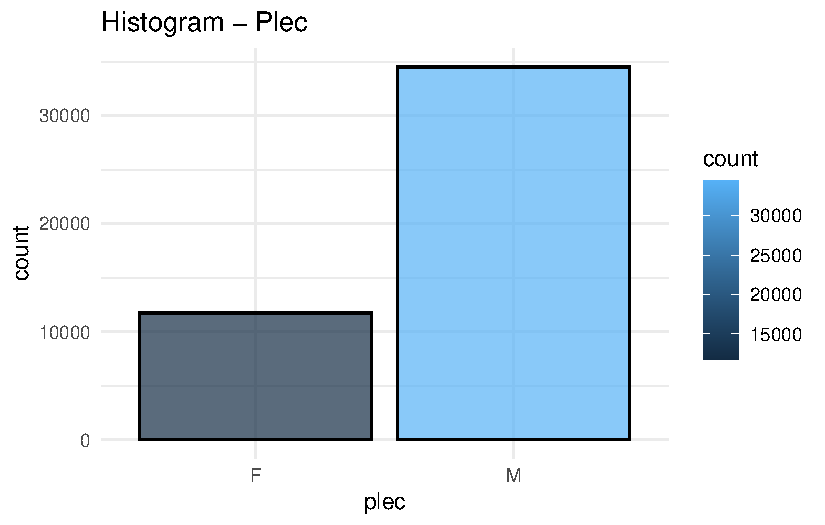
\includegraphics{raport_files/figure-pdf/unnamed-chunk-10-1.pdf}

}

\caption{Histogram zmiennej - Płeć}

}

\end{minipage}%
%
\begin{minipage}[t]{0.50\linewidth}

{\centering 

\begin{longtable}[]{@{}lrr@{}}
\caption{Tabela przedstawiająca liczność i procent pod względem płci
}\tabularnewline
\toprule\noalign{}
Plec & Licznosc & Procent \\
\midrule\noalign{}
\endfirsthead
\toprule\noalign{}
Plec & Licznosc & Procent \\
\midrule\noalign{}
\endhead
\bottomrule\noalign{}
\endlastfoot
F & 11748 & 25.4 \\
M & 34510 & 74.6 \\
\end{longtable}

}

\end{minipage}%
\newline
\begin{minipage}[t]{0.50\linewidth}

{\centering 

Histogram zmiennej - Płeć

}

\end{minipage}%

\end{figure}

\hypertarget{zmienna-kategoria-wiekowa}{%
\subsection{\texorpdfstring{3.2 Zmienna: \emph{Kategoria
wiekowa}}{3.2 Zmienna: Kategoria wiekowa}}\label{zmienna-kategoria-wiekowa}}

Występuje tutaj 16 różnych wartości, przypisujących danego zawodnika do
danej kategorii. Najwięcej osób startuje w kategorii wiekowej
\emph{24-34}, co stanowi ok. 29\% wszystkich zawodników. Kategorię
\emph{80-999} należy rozumieć jako osoby w wieku \(\ge 80\)

\begin{Shaded}
\begin{Highlighting}[]
\NormalTok{desired\_order }\OtherTok{=} \FunctionTok{c}\NormalTok{(}\StringTok{"5{-}12"}\NormalTok{, }\StringTok{"13{-}15"}\NormalTok{, }\StringTok{"16{-}17"}\NormalTok{, }\StringTok{"18{-}19"}\NormalTok{, }\StringTok{"20{-}23"}\NormalTok{, }\StringTok{"24{-}34"}\NormalTok{, }\StringTok{"35{-}39"}\NormalTok{, }\StringTok{"40{-}44"}\NormalTok{, }\StringTok{"45{-}49"}\NormalTok{, }\StringTok{"50{-}54"}\NormalTok{, }\StringTok{"55{-}59"}\NormalTok{, }\StringTok{"60{-}64"}\NormalTok{, }\StringTok{"65{-}69"}\NormalTok{, }\StringTok{"70{-}74"}\NormalTok{, }\StringTok{"75{-}79"}\NormalTok{, }\StringTok{"80{-}999"}\NormalTok{)}

\FunctionTok{ggplot}\NormalTok{(probka, }\FunctionTok{aes}\NormalTok{(}\AttributeTok{x =}\NormalTok{ wiek, }\AttributeTok{y =}\NormalTok{ ..count.., }\AttributeTok{fill =}\NormalTok{ ..count..)) }\SpecialCharTok{+}
  \FunctionTok{geom\_bar}\NormalTok{(}\AttributeTok{color =} \StringTok{"black"}\NormalTok{, }\AttributeTok{alpha =} \FloatTok{0.7}\NormalTok{, }\AttributeTok{position =} \StringTok{"identity"}\NormalTok{) }\SpecialCharTok{+}
  \FunctionTok{labs}\NormalTok{(}\AttributeTok{title =} \StringTok{"Histogram {-} Wiek"}\NormalTok{, }\AttributeTok{x =} \StringTok{"wiek"}\NormalTok{, }\AttributeTok{y =} \StringTok{"ilość"}\NormalTok{) }\SpecialCharTok{+}
  \FunctionTok{scale\_x\_discrete}\NormalTok{(}\AttributeTok{limits =}\NormalTok{ desired\_order) }\SpecialCharTok{+} 
  \FunctionTok{theme\_minimal}\NormalTok{()}
\NormalTok{wiek\_ilosc }\OtherTok{\textless{}{-}} \FunctionTok{table}\NormalTok{(probka}\SpecialCharTok{$}\NormalTok{wiek)}
\NormalTok{procent\_danych }\OtherTok{\textless{}{-}}  \FunctionTok{round}\NormalTok{(}\FunctionTok{prop.table}\NormalTok{(wiek\_ilosc) }\SpecialCharTok{*} \DecValTok{100}\NormalTok{, }\AttributeTok{digits=}\DecValTok{2}\NormalTok{)}
\NormalTok{stats }\OtherTok{\textless{}{-}} \FunctionTok{data.frame}\NormalTok{(}\AttributeTok{Wiek =} \FunctionTok{as.character}\NormalTok{(}\FunctionTok{names}\NormalTok{(wiek\_ilosc)), }\AttributeTok{Licznosc =} \FunctionTok{as.numeric}\NormalTok{(wiek\_ilosc), }\AttributeTok{Procent =} \FunctionTok{as.numeric}\NormalTok{(procent\_danych))}

\NormalTok{knitr}\SpecialCharTok{::}\FunctionTok{kable}\NormalTok{(stats)}
\end{Highlighting}
\end{Shaded}

\begin{figure}

\begin{minipage}[t]{0.50\linewidth}

{\centering 

\raisebox{-\height}{

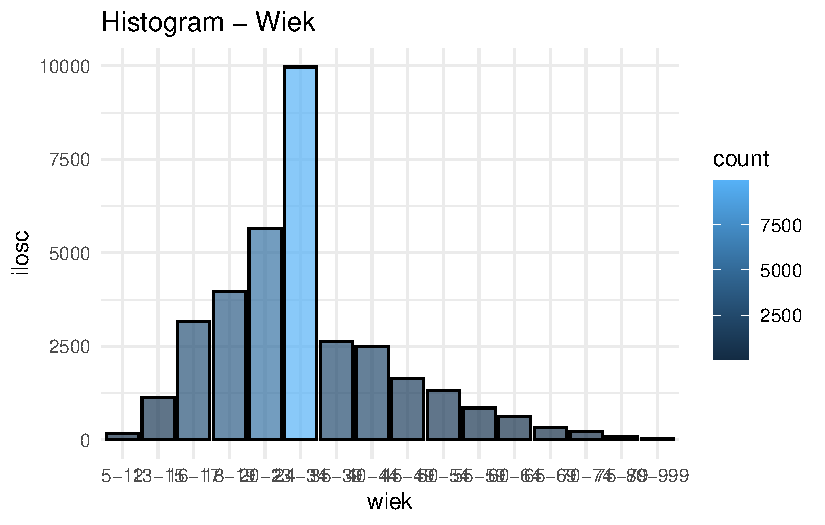
\includegraphics{raport_files/figure-pdf/unnamed-chunk-11-1.pdf}

}

\caption{Histogram zmiennej - Kategoria wiekowa}

}

\end{minipage}%
%
\begin{minipage}[t]{0.50\linewidth}

{\centering 

\begin{longtable}[]{@{}lrr@{}}
\caption{Tabela przedstawiająca liczność i procent dla danej kategorii
wiekowej }\tabularnewline
\toprule\noalign{}
Wiek & Licznosc & Procent \\
\midrule\noalign{}
\endfirsthead
\toprule\noalign{}
Wiek & Licznosc & Procent \\
\midrule\noalign{}
\endhead
\bottomrule\noalign{}
\endlastfoot
& 11966 & 25.87 \\
13-15 & 1134 & 2.45 \\
16-17 & 3160 & 6.83 \\
18-19 & 3960 & 8.56 \\
20-23 & 5644 & 12.20 \\
24-34 & 9973 & 21.56 \\
35-39 & 2637 & 5.70 \\
40-44 & 2493 & 5.39 \\
45-49 & 1637 & 3.54 \\
5-12 & 171 & 0.37 \\
50-54 & 1321 & 2.86 \\
55-59 & 854 & 1.85 \\
60-64 & 623 & 1.35 \\
65-69 & 338 & 0.73 \\
70-74 & 220 & 0.48 \\
75-79 & 91 & 0.20 \\
80-999 & 36 & 0.08 \\
\end{longtable}

}

\end{minipage}%
\newline
\begin{minipage}[t]{0.50\linewidth}

{\centering 

Histogram zmiennej - Kategoria wiekowa

}

\end{minipage}%

\end{figure}

\hypertarget{zmienna-waga-zawodnika}{%
\subsection{\texorpdfstring{3.3 Zmienna: \emph{Waga
zawodnika}}{3.3 Zmienna: Waga zawodnika}}\label{zmienna-waga-zawodnika}}

Dla tej zmiennej ciągłej można już przeprowadzić szereg analiz
statystycznych oraz narysować wykres pudełkowy.

\begin{Shaded}
\begin{Highlighting}[]
\FunctionTok{ggplot}\NormalTok{(probka, }\FunctionTok{aes}\NormalTok{(}\AttributeTok{x =}\NormalTok{ masa, }\AttributeTok{y =}\NormalTok{ ..density.., }\AttributeTok{fill =}\NormalTok{ ..density..)) }\SpecialCharTok{+}
  \FunctionTok{geom\_histogram}\NormalTok{(}\AttributeTok{binwidth =} \DecValTok{7}\NormalTok{, }\AttributeTok{color =} \StringTok{"black"}\NormalTok{, }\AttributeTok{alpha =} \FloatTok{0.7}\NormalTok{, }\AttributeTok{position =} \StringTok{"identity"}\NormalTok{) }\SpecialCharTok{+}
  \FunctionTok{ggtitle}\NormalTok{(}\StringTok{"Unormowany histogram {-} Masa zawodnika"}\NormalTok{) }\SpecialCharTok{+}
  \FunctionTok{theme\_minimal}\NormalTok{() }\SpecialCharTok{+}
  \FunctionTok{scale\_y\_continuous}\NormalTok{(}\AttributeTok{labels =}\NormalTok{ scales}\SpecialCharTok{::}\FunctionTok{percent\_format}\NormalTok{(}\AttributeTok{scale =} \DecValTok{1}\NormalTok{))}

\FunctionTok{ggplot}\NormalTok{(probka, }\FunctionTok{aes}\NormalTok{(}\AttributeTok{y =}\NormalTok{ masa)) }\SpecialCharTok{+}
  \FunctionTok{geom\_boxplot}\NormalTok{() }\SpecialCharTok{+}
  \FunctionTok{ggtitle}\NormalTok{(}\StringTok{"Wykres pudełkowy masy"}\NormalTok{) }\SpecialCharTok{+}
  \FunctionTok{theme\_minimal}\NormalTok{()}
\end{Highlighting}
\end{Shaded}

\begin{figure}

\begin{minipage}[t]{0.50\linewidth}

{\centering 

\raisebox{-\height}{

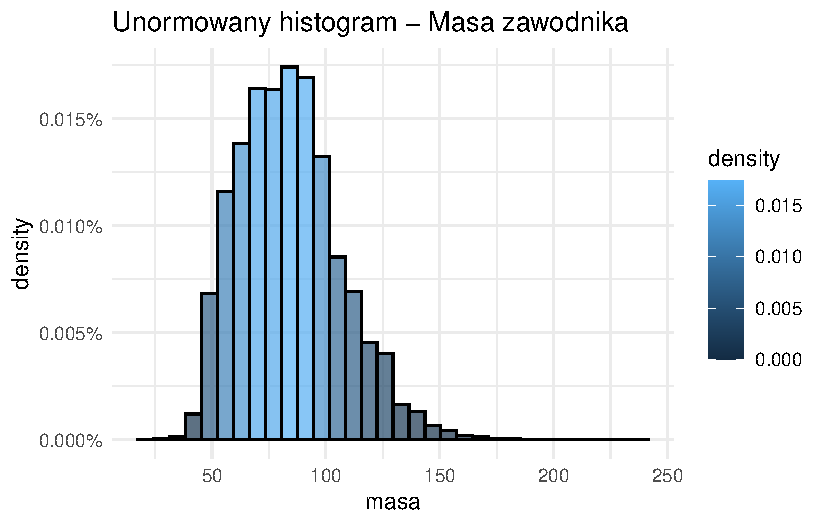
\includegraphics{raport_files/figure-pdf/unnamed-chunk-12-1.pdf}

}

\caption{Histogram}

}

\end{minipage}%
%
\begin{minipage}[t]{0.50\linewidth}

{\centering 

\raisebox{-\height}{

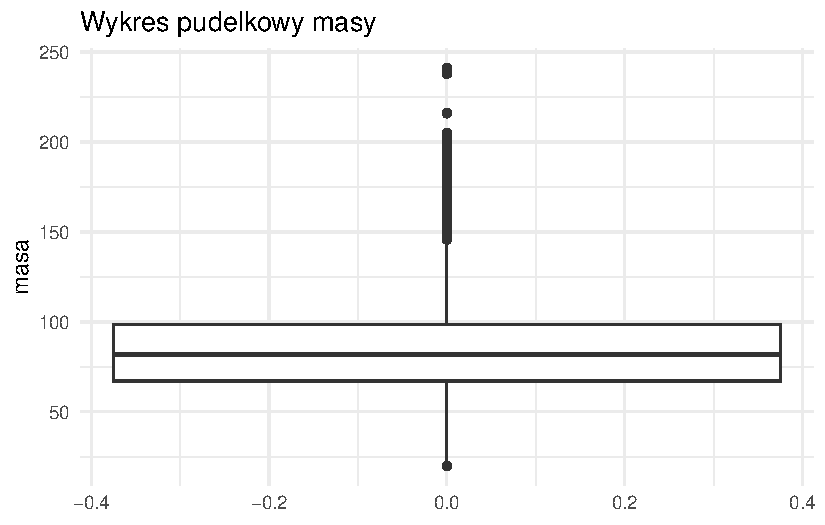
\includegraphics{raport_files/figure-pdf/unnamed-chunk-12-2.pdf}

}

\caption{Boxplot}

}

\end{minipage}%
\newline
\begin{minipage}[t]{0.50\linewidth}

{\centering 

Wykresy dla zmiennej Masa

}

\end{minipage}%

\end{figure}

Na histogramie widzimy, że jest on prawostronnie skośny i prawie
symetryczny. Ponadto zarówno histogram, jak i wykres pudełkowy wykazują
dużą obecność tzw. outliersów, czyli wartości odstających, wywołanych
niskim rozstępem międzykwartylowym. Wysoka intensywność występowania
wartości skrajnych może sugerować dodatnią kurtozę nadwyżkową. Poniżej w
tabeli przedstawione są podstawowe statystki dla tej zmiennej.

\begin{Shaded}
\begin{Highlighting}[]
\NormalTok{summary\_df }\OtherTok{\textless{}{-}} \FunctionTok{data.frame}\NormalTok{(}
  \AttributeTok{Statystyki =} \FunctionTok{c}\NormalTok{(}\StringTok{"Minimum"}\NormalTok{, }\StringTok{"Pierwszy kwartyl"}\NormalTok{, }\StringTok{"Mediana"}\NormalTok{, }\StringTok{"Srednia"}\NormalTok{, }\StringTok{"Trzeci kwartyl"}\NormalTok{, }\StringTok{"Rozstep miedzykwartylowy"}\NormalTok{, }\StringTok{"Maximum"}\NormalTok{, }\StringTok{"Wariancja"}\NormalTok{, }\StringTok{"Skosnosc"}\NormalTok{, }\StringTok{"Kurtoza nadwyżkowa"}\NormalTok{),}
  \AttributeTok{Wartosci =} \FunctionTok{c}\NormalTok{(}\FunctionTok{min}\NormalTok{(probka}\SpecialCharTok{$}\NormalTok{masa), }\FunctionTok{quantile}\NormalTok{(probka}\SpecialCharTok{$}\NormalTok{masa, }\FloatTok{0.25}\NormalTok{), }\FunctionTok{median}\NormalTok{(probka}\SpecialCharTok{$}\NormalTok{masa), }\FunctionTok{mean}\NormalTok{(probka}\SpecialCharTok{$}\NormalTok{masa), }\FunctionTok{quantile}\NormalTok{(probka}\SpecialCharTok{$}\NormalTok{masa, }\FloatTok{0.75}\NormalTok{), }\FunctionTok{IQR}\NormalTok{(probka}\SpecialCharTok{$}\NormalTok{masa), }\FunctionTok{max}\NormalTok{(probka}\SpecialCharTok{$}\NormalTok{masa), }\FunctionTok{var}\NormalTok{(probka}\SpecialCharTok{$}\NormalTok{masa), }\FunctionTok{skewness}\NormalTok{(probka}\SpecialCharTok{$}\NormalTok{masa), }\FunctionTok{kurtosis}\NormalTok{(probka}\SpecialCharTok{$}\NormalTok{masa))}
\NormalTok{)}

\NormalTok{knitr}\SpecialCharTok{::}\FunctionTok{kable}\NormalTok{(summary\_df)}
\end{Highlighting}
\end{Shaded}

\begin{longtable}[]{@{}lr@{}}
\caption{Tabela przedstawiająca zbiór wartości poszczególnych statystyk
}\tabularnewline
\toprule\noalign{}
Statystyki & Wartosci \\
\midrule\noalign{}
\endfirsthead
\toprule\noalign{}
Statystyki & Wartosci \\
\midrule\noalign{}
\endhead
\bottomrule\noalign{}
\endlastfoot
Minimum & 20.0000000 \\
Pierwszy kwartyl & 67.2000000 \\
Mediana & 81.8000000 \\
Srednia & 83.9864408 \\
Trzeci kwartyl & 98.6000000 \\
Rozstep miedzykwartylowy & 31.4000000 \\
Maximum & 241.1000000 \\
Wariancja & 505.7357659 \\
Skosnosc & 0.6726162 \\
Kurtoza nadwyżkowa & 0.6523304 \\
\end{longtable}

Wartość mediany jest zbliżona do wartości średniej, co wskazuje na dość
dużą symetryczność rozkładu. Brak ich pokrycia wynika z istnienia
wartości odstających. Skośność większa od 0 wskazuje na prawoskośność,
co zgadza się z wnioskami odnośnie histogramu oraz jego wyglądem.
Kurtoza nadwyżkowa większa od 0 oznacza, że rozkład jest leptokurtyczny.
Istnieje jednak wiele podobieństw pomiędzy rozkładem mas zawodników oraz
rozkładem normalnym. Rozbieżność występuje prawdopodobnie ze względu na
niestandardowe warunki, którymi są zawody w trójboju siłowym. Zbiorem
danych są sportowcy, a nie losowa grupa ludzi, przez co rozkład masy
zawodników może bardziej różnić się od rozkładu normalnego, niż losowa
próba z populacji.

\hypertarget{zmienna-total}{%
\subsection{\texorpdfstring{3.4 Zmienna:
\emph{Total}}{3.4 Zmienna: Total}}\label{zmienna-total}}

Dla tej zmiennej ciągłej również możemy narysować histogram, wykres
pudełkowy oraz policzyć wartości wybranych statystyk.

\begin{Shaded}
\begin{Highlighting}[]
\FunctionTok{ggplot}\NormalTok{(probka, }\FunctionTok{aes}\NormalTok{(}\AttributeTok{x =}\NormalTok{ total, }\AttributeTok{y =}\NormalTok{ ..density.., }\AttributeTok{fill =}\NormalTok{ ..density..)) }\SpecialCharTok{+}
  \FunctionTok{geom\_histogram}\NormalTok{(}\AttributeTok{binwidth =} \DecValTok{20}\NormalTok{, }\AttributeTok{color =} \StringTok{"black"}\NormalTok{, }\AttributeTok{alpha =} \FloatTok{0.7}\NormalTok{, }\AttributeTok{position =} \StringTok{"identity"}\NormalTok{) }\SpecialCharTok{+}
  \FunctionTok{ggtitle}\NormalTok{(}\StringTok{"Unormowany histogram {-} Suma wszystkich podniesionych ciężarów"}\NormalTok{) }\SpecialCharTok{+}
  \FunctionTok{theme\_minimal}\NormalTok{() }\SpecialCharTok{+}
  \FunctionTok{scale\_y\_continuous}\NormalTok{(}\AttributeTok{labels =}\NormalTok{ scales}\SpecialCharTok{::}\FunctionTok{percent\_format}\NormalTok{(}\AttributeTok{scale =} \DecValTok{1}\NormalTok{))}

\FunctionTok{ggplot}\NormalTok{(probka, }\FunctionTok{aes}\NormalTok{(}\AttributeTok{y =}\NormalTok{ total)) }\SpecialCharTok{+}
  \FunctionTok{geom\_boxplot}\NormalTok{() }\SpecialCharTok{+}
  \FunctionTok{ggtitle}\NormalTok{(}\StringTok{"Wykres pudełkowy wyniku total"}\NormalTok{) }\SpecialCharTok{+}
  \FunctionTok{theme\_minimal}\NormalTok{()}
\end{Highlighting}
\end{Shaded}

\begin{figure}

\begin{minipage}[t]{0.50\linewidth}

{\centering 

\raisebox{-\height}{

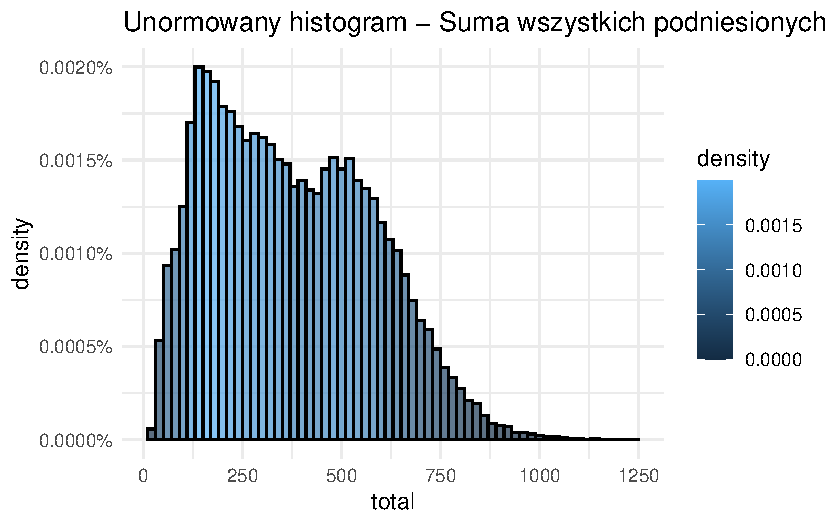
\includegraphics{raport_files/figure-pdf/unnamed-chunk-14-1.pdf}

}

\caption{Histogram}

}

\end{minipage}%
%
\begin{minipage}[t]{0.50\linewidth}

{\centering 

\raisebox{-\height}{

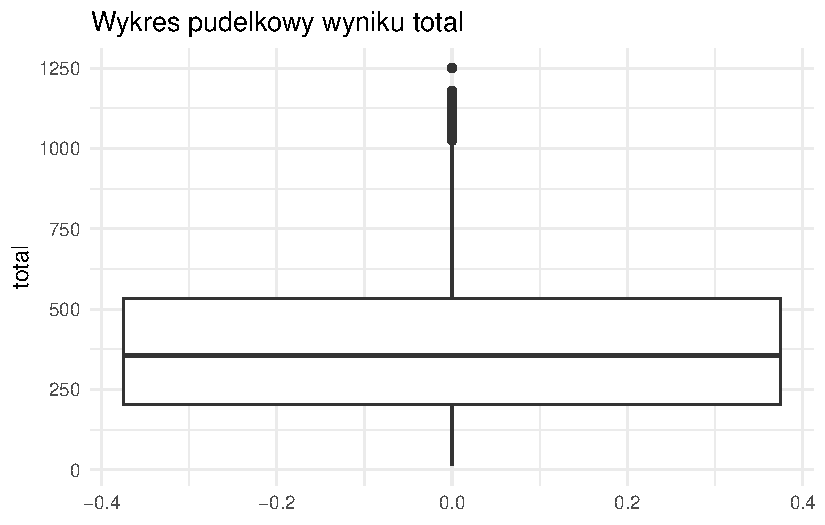
\includegraphics{raport_files/figure-pdf/unnamed-chunk-14-2.pdf}

}

\caption{Boxplot}

}

\end{minipage}%
\newline
\begin{minipage}[t]{0.50\linewidth}

{\centering 

Wykresy dla zmiennej Total

}

\end{minipage}%

\end{figure}

Na boxplocie widzimy znacznie mniej wartości odstających, niż dla
zmiennej \textbf{masa}. Jest to spowodowane większą koncentracją danych
i zwiększeniem rozstępu międzykwartylowego - zawodnicy są na podobnym
poziomie, z pojedynczymi jednostkami wybitnymi. Histogram przypomina
rozkład prawoskośny i jest niesymetryczny ze względu na swoje dwa
\emph{szczyty.}

\begin{Shaded}
\begin{Highlighting}[]
\NormalTok{summary\_df }\OtherTok{\textless{}{-}} \FunctionTok{data.frame}\NormalTok{(}
  \AttributeTok{Statystyki =} \FunctionTok{c}\NormalTok{(}\StringTok{"Minimum"}\NormalTok{, }\StringTok{"Pierwszy kwartyl"}\NormalTok{, }\StringTok{"Mediana"}\NormalTok{, }\StringTok{"Srednia"}\NormalTok{, }\StringTok{"Trzeci kwartyl"}\NormalTok{, }\StringTok{"Rozstep miedzykwartylowy"}\NormalTok{, }\StringTok{"Maximum"}\NormalTok{, }\StringTok{"Wariancja"}\NormalTok{, }\StringTok{"Skosnosc"}\NormalTok{, }\StringTok{"Kurtoza nadwyżkowa"}\NormalTok{),}
  \AttributeTok{Wartosci =} \FunctionTok{c}\NormalTok{(}\FunctionTok{min}\NormalTok{(probka}\SpecialCharTok{$}\NormalTok{total), }\FunctionTok{quantile}\NormalTok{(probka}\SpecialCharTok{$}\NormalTok{total, }\FloatTok{0.25}\NormalTok{), }\FunctionTok{median}\NormalTok{(probka}\SpecialCharTok{$}\NormalTok{total), }\FunctionTok{mean}\NormalTok{(probka}\SpecialCharTok{$}\NormalTok{total), }\FunctionTok{quantile}\NormalTok{(probka}\SpecialCharTok{$}\NormalTok{total, }\FloatTok{0.75}\NormalTok{), }\FunctionTok{IQR}\NormalTok{(probka}\SpecialCharTok{$}\NormalTok{total), }\FunctionTok{max}\NormalTok{(probka}\SpecialCharTok{$}\NormalTok{total), }\FunctionTok{var}\NormalTok{(probka}\SpecialCharTok{$}\NormalTok{total), }\FunctionTok{skewness}\NormalTok{(probka}\SpecialCharTok{$}\NormalTok{total), }\FunctionTok{kurtosis}\NormalTok{(probka}\SpecialCharTok{$}\NormalTok{total))}
\NormalTok{)}
\NormalTok{knitr}\SpecialCharTok{::}\FunctionTok{kable}\NormalTok{(summary\_df)}
\end{Highlighting}
\end{Shaded}

\begin{longtable}[]{@{}lr@{}}
\caption{Tabela przedstawiająca zbiór wartości poszczególnych statystyk
}\tabularnewline
\toprule\noalign{}
Statystyki & Wartosci \\
\midrule\noalign{}
\endfirsthead
\toprule\noalign{}
Statystyki & Wartosci \\
\midrule\noalign{}
\endhead
\bottomrule\noalign{}
\endlastfoot
Minimum & 12.5000000 \\
Pierwszy kwartyl & 204.1200000 \\
Mediana & 356.0700000 \\
Srednia & 378.2211678 \\
Trzeci kwartyl & 532.5000000 \\
Rozstep miedzykwartylowy & 328.3800000 \\
Maximum & 1250.0000000 \\
Wariancja & 41887.4868748 \\
Skosnosc & 0.3981495 \\
Kurtoza nadwyżkowa & -0.6074609 \\
\end{longtable}

Wartość mediany jest ponownie zbliżona do średniej, jednak wygląd
histogramu wyklucza symetryczność~rozkładu. Skośność, podobnie jak dla
\textbf{masy} jest większa od 0, potwierdzając prawoskośność. Kurtoza
nadwyżkowa tym razem spada poniżej zera, co oznacza platykurtyczność. W
wypadku tych danych można odrzucić hipotezę o podobieństwie do rozkładu
normalnego. Powodów może być kilka, przy czym najbardziej przekonującym
jest zróżnicowanie. Wybieramy spośród sportowców, którzy mają różne
programy treningowe, różne możliwości fizyczne, podantości na kontuzje,
zdolności. Dodatkowo analizujemy tylko i wyłącznie tych, którzy
konkurują w podnosieniu ciężarów. Prawdopodobnie inaczej wyglądałby
wykres, gdyby móc przeanalizować dane dla \emph{wszystkich} trójboistów
- znacznie inaczej, gdyby przeanalizować również dane ludzi, którzy
trójboju nie trenują. Ponadto dłuższy jest prawy ogon, ponieważ w
trójboju raczej częściej będą zdarzać się jednostki wybitne, niż
tragiczne. Wszyscy zadownicy są na podobnym poziomie, a jeśli już zdarzy
się jakaś wartość odstająca, to raczej będzie lepsza od reszty, niż
gorsza.

\hypertarget{rozkux142ady-warunkowe}{%
\section{4. Rozkłady warunkowe}\label{rozkux142ady-warunkowe}}

\hypertarget{rozkux142ady-zmiennych-warunkowane-pux142ciux105}{%
\subsection{4.1. Rozkłady zmiennych warunkowane
płcią}\label{rozkux142ady-zmiennych-warunkowane-pux142ciux105}}

Na wykresach poniżej znajdują się rozkłady zmiennych \textbf{Masa} oraz
\textbf{Total} warunkowane zmienną \textbf{Płeć.} Z wykresów możemy
zauważyć ewidentną \textbf{bimodalność} zmiennej \textbf{Total} dla
określonej płci.

\begin{Shaded}
\begin{Highlighting}[]
\FunctionTok{ggplot}\NormalTok{(probka, }\FunctionTok{aes}\NormalTok{(}\AttributeTok{x =}\NormalTok{ masa, }\AttributeTok{y =}\NormalTok{ ..density.., }\AttributeTok{fill =}\NormalTok{ ..density..)) }\SpecialCharTok{+}
  \FunctionTok{geom\_histogram}\NormalTok{(}\AttributeTok{binwidth =} \DecValTok{7}\NormalTok{, }\AttributeTok{color =} \StringTok{"black"}\NormalTok{, }\AttributeTok{alpha =} \FloatTok{0.7}\NormalTok{, }\AttributeTok{position =} \StringTok{"identity"}\NormalTok{) }\SpecialCharTok{+}
  \FunctionTok{ggtitle}\NormalTok{(}\StringTok{"Histogram {-} Masa"}\NormalTok{) }\SpecialCharTok{+}
  \FunctionTok{theme\_minimal}\NormalTok{() }\SpecialCharTok{+}
  \FunctionTok{facet\_grid}\NormalTok{(plec }\SpecialCharTok{\textasciitilde{}}\NormalTok{ ., }\AttributeTok{scales =} \StringTok{"free\_y"}\NormalTok{) }\SpecialCharTok{+}
  \FunctionTok{scale\_y\_continuous}\NormalTok{(}\AttributeTok{labels =}\NormalTok{ scales}\SpecialCharTok{::}\FunctionTok{percent\_format}\NormalTok{(}\AttributeTok{scale =} \DecValTok{1}\NormalTok{))}

\FunctionTok{ggplot}\NormalTok{(probka, }\FunctionTok{aes}\NormalTok{(}\AttributeTok{x =}\NormalTok{ total, }\AttributeTok{y =}\NormalTok{ ..density.., }\AttributeTok{fill =}\NormalTok{ ..density..)) }\SpecialCharTok{+}
  \FunctionTok{geom\_histogram}\NormalTok{(}\AttributeTok{binwidth =} \DecValTok{20}\NormalTok{, }\AttributeTok{color =} \StringTok{"black"}\NormalTok{, }\AttributeTok{alpha =} \FloatTok{0.7}\NormalTok{, }\AttributeTok{position =} \StringTok{"identity"}\NormalTok{) }\SpecialCharTok{+}
  \FunctionTok{ggtitle}\NormalTok{(}\StringTok{"Histogram {-} Total"}\NormalTok{) }\SpecialCharTok{+}
  \FunctionTok{theme\_minimal}\NormalTok{() }\SpecialCharTok{+}
  \FunctionTok{facet\_grid}\NormalTok{(plec }\SpecialCharTok{\textasciitilde{}}\NormalTok{ ., }\AttributeTok{scales =} \StringTok{"free\_y"}\NormalTok{) }\SpecialCharTok{+}
  \FunctionTok{scale\_y\_continuous}\NormalTok{(}\AttributeTok{labels =}\NormalTok{ scales}\SpecialCharTok{::}\FunctionTok{percent\_format}\NormalTok{(}\AttributeTok{scale =} \DecValTok{1}\NormalTok{))}
\end{Highlighting}
\end{Shaded}

\begin{figure}

\begin{minipage}[t]{0.50\linewidth}

{\centering 

\raisebox{-\height}{

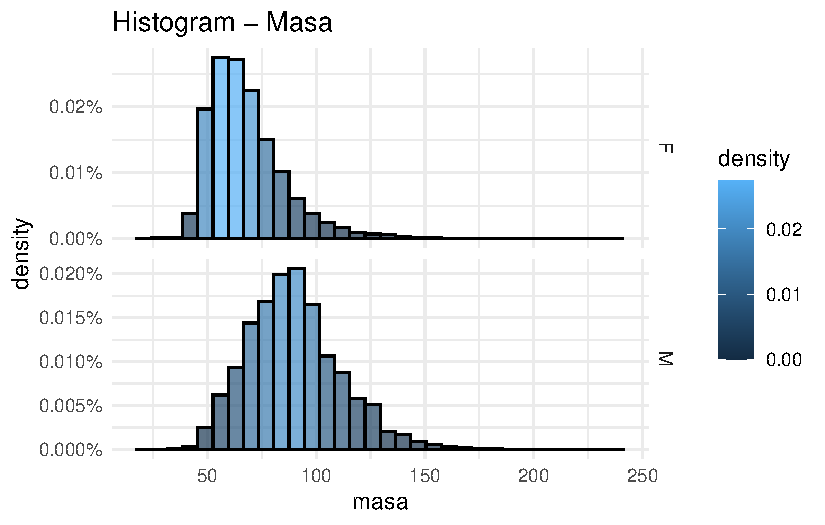
\includegraphics{raport_files/figure-pdf/unnamed-chunk-16-1.pdf}

}

\caption{Masa}

}

\end{minipage}%
%
\begin{minipage}[t]{0.50\linewidth}

{\centering 

\raisebox{-\height}{

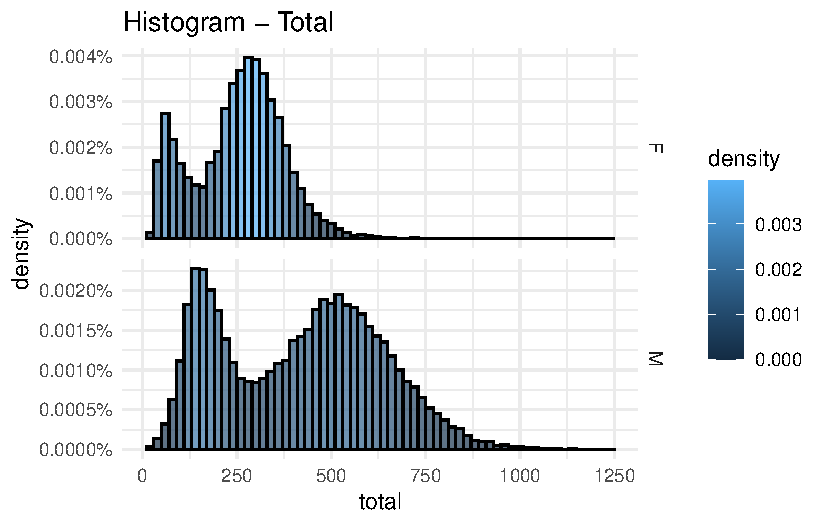
\includegraphics{raport_files/figure-pdf/unnamed-chunk-16-2.pdf}

}

\caption{Total}

}

\end{minipage}%
\newline
\begin{minipage}[t]{0.50\linewidth}

{\centering 

Histogramy masy zawodnika i jego wyniku dla poszczególnych płci

}

\end{minipage}%

\end{figure}

\hypertarget{rozkux142ady-zmiennych-warunkowane-wiekiem.}{%
\subsection{4.2. Rozkłady zmiennych warunkowane
wiekiem.}\label{rozkux142ady-zmiennych-warunkowane-wiekiem.}}

Na poniższych wykresach pudełkowych przedstawione są rozkłady zmiennych
\textbf{Masa} i \textbf{Total} warunkowane zmienną \textbf{Wiek.}

\begin{Shaded}
\begin{Highlighting}[]
\FunctionTok{ggplot}\NormalTok{(probka, }\FunctionTok{aes}\NormalTok{(}\AttributeTok{x =}\NormalTok{ wiek, }\AttributeTok{y =}\NormalTok{ masa, }\AttributeTok{fill =}\NormalTok{ wiek)) }\SpecialCharTok{+}
  \FunctionTok{geom\_boxplot}\NormalTok{() }\SpecialCharTok{+}
  \FunctionTok{ggtitle}\NormalTok{(}\StringTok{"Wykresy pudełkowe masy warunkowanej wiekiem"}\NormalTok{) }\SpecialCharTok{+}
  \FunctionTok{scale\_x\_discrete}\NormalTok{(}\AttributeTok{limits =}\NormalTok{ desired\_order) }\SpecialCharTok{+} 
  \FunctionTok{theme\_minimal}\NormalTok{()}

\FunctionTok{ggplot}\NormalTok{(probka, }\FunctionTok{aes}\NormalTok{(}\AttributeTok{x =}\NormalTok{ wiek, }\AttributeTok{y =}\NormalTok{ total, }\AttributeTok{fill =}\NormalTok{ wiek)) }\SpecialCharTok{+}
  \FunctionTok{geom\_boxplot}\NormalTok{() }\SpecialCharTok{+}
  \FunctionTok{ggtitle}\NormalTok{(}\StringTok{"Wykresy pudełkowe wyniku total warunkowanego wiekiem"}\NormalTok{) }\SpecialCharTok{+}
  \FunctionTok{scale\_x\_discrete}\NormalTok{(}\AttributeTok{limits =}\NormalTok{ desired\_order) }\SpecialCharTok{+} 
  \FunctionTok{theme\_minimal}\NormalTok{()}
\end{Highlighting}
\end{Shaded}

\begin{figure}

\begin{minipage}[t]{0.50\linewidth}

{\centering 

\raisebox{-\height}{

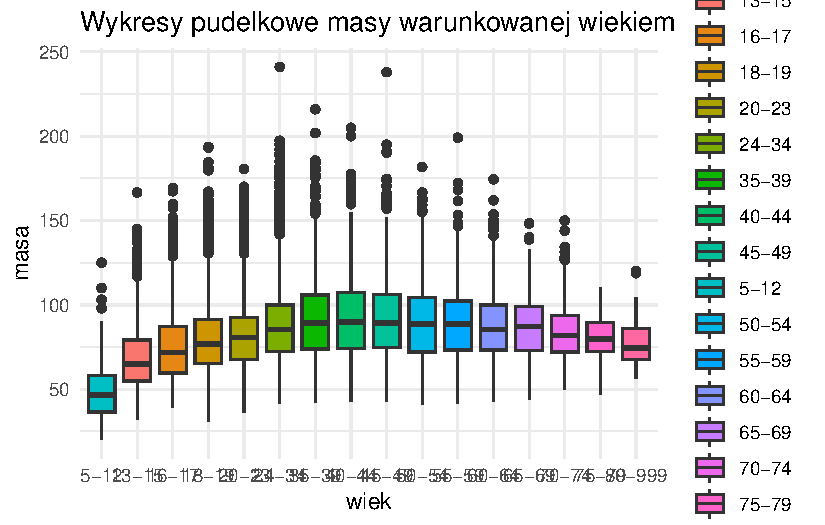
\includegraphics{raport_files/figure-pdf/unnamed-chunk-17-1.pdf}

}

\caption{Masa}

}

\end{minipage}%
%
\begin{minipage}[t]{0.50\linewidth}

{\centering 

\raisebox{-\height}{

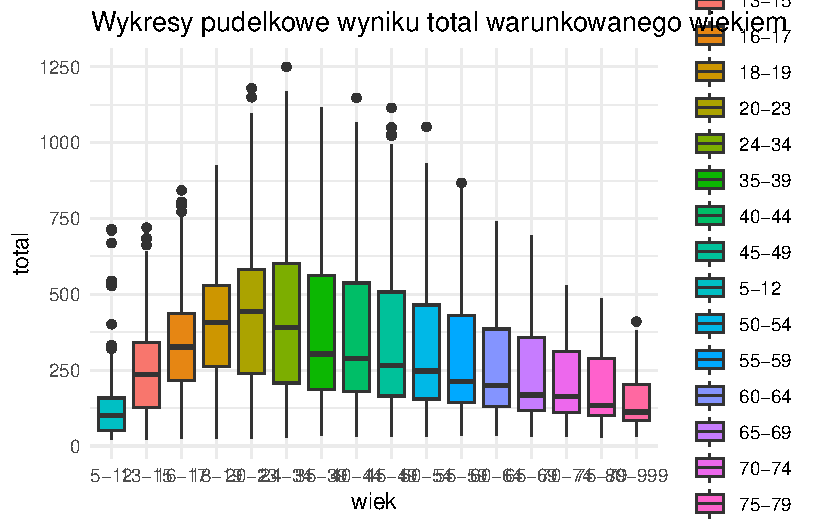
\includegraphics{raport_files/figure-pdf/unnamed-chunk-17-2.pdf}

}

\caption{Total}

}

\end{minipage}%
\newline
\begin{minipage}[t]{0.50\linewidth}

{\centering 

Wykresy pudełkowe masy zawodnika i jego wyniku dla poszczególnych
przedziałów

}

\end{minipage}%

\end{figure}

\hypertarget{wynik-total-a-wiek.}{%
\subsubsection{4.2.1. Wynik total a wiek.}\label{wynik-total-a-wiek.}}

Przypatrując się rozkładom zmiennej \textbf{Total} widzimy, że górne
wąsy są znacznie dłuższe od dolnych oraz, że mediana jest bliżej
pierwszego kwartyla. Dodatkowo różnice te zdają się narastać z wiekiem.
Możemy zatem wywnioskować znaczną prawostronną skośność zmiennej
\textbf{Total} warunkowanej \textbf{Wiekiem.} Dodatkowo skośność ta
zwiększa się wraz ze wzrostem wieku. Potwierdza się to w danych z
poniższej tabeli.

\begin{Shaded}
\begin{Highlighting}[]
\NormalTok{wiek\_ilosc }\OtherTok{\textless{}{-}} \FunctionTok{table}\NormalTok{(probka}\SpecialCharTok{$}\NormalTok{wiek)}

\NormalTok{stats }\OtherTok{\textless{}{-}}\NormalTok{ probka }\SpecialCharTok{\%\textgreater{}\%} \FunctionTok{group\_by}\NormalTok{(wiek) }\SpecialCharTok{\%\textgreater{}\%} \FunctionTok{summarize}\NormalTok{(}\AttributeTok{Skosnosc =} \FunctionTok{skewness}\NormalTok{(total), }\AttributeTok{Kurtoza\_nadwyzkowa =} \FunctionTok{kurtosis}\NormalTok{(total))}

\NormalTok{knitr}\SpecialCharTok{::}\FunctionTok{kable}\NormalTok{(stats)}
\end{Highlighting}
\end{Shaded}

\begin{longtable}[]{@{}lrr@{}}
\caption{Tabela przedstawiająca skośność i kurtozę rozkładu wyniku total
warunkowanego wiekiem }\tabularnewline
\toprule\noalign{}
wiek & Skosnosc & Kurtoza\_nadwyzkowa \\
\midrule\noalign{}
\endfirsthead
\toprule\noalign{}
wiek & Skosnosc & Kurtoza\_nadwyzkowa \\
\midrule\noalign{}
\endhead
\bottomrule\noalign{}
\endlastfoot
& 0.2780792 & -0.4331673 \\
13-15 & 0.3746677 & -0.4525842 \\
16-17 & 0.0793386 & -0.5930804 \\
18-19 & -0.1033734 & -0.7966307 \\
20-23 & 0.0521875 & -0.8783159 \\
24-34 & 0.3216442 & -0.9021865 \\
35-39 & 0.6204089 & -0.6613723 \\
40-44 & 0.6433957 & -0.6440888 \\
45-49 & 0.7545083 & -0.3772775 \\
5-12 & 2.4121606 & 6.6358645 \\
50-54 & 0.7592848 & -0.4474953 \\
55-59 & 0.8461354 & -0.4060648 \\
60-64 & 0.7555853 & -0.5720298 \\
65-69 & 0.8043215 & -0.5803235 \\
70-74 & 0.7688846 & -0.6465690 \\
75-79 & 0.9158347 & -0.5115341 \\
80-999 & 1.1965920 & 0.4847552 \\
\end{longtable}

\hypertarget{masa-a-wiek.}{%
\subsubsection{4.2.2. Masa a wiek.}\label{masa-a-wiek.}}

Patrząc zaś na boxploty opisujące \textbf{masę} zawodnika widzimy wiele
wartości skrajnych większych niż \(Q_3 + 1,5\,\text{IQR}\) co jest
przesłanką ku leptokurtyczności rozkładów warunkowych. Potwierdza się to
w poniższej tabeli. Zjawisko to ma prostą interpretację. Otóż we
wszystkich zawodach trójbojowych stosuje się \textbf{kategorie wagowe}
aby zwodnicy konkurowali z rywalami do siebie podobnymi\textbf{.}
Ostatnią kategorią są zazwykle kategorie typu 120+, 140+, które nie
posiadają kresu górnego. Tym samym u tych zawodników optymalne jest
posiadanie jak największej masy ciała aby zyskać przewagę nad rywalami.
Powoduje to częste występowanie wartości skrajnych. Z wykresu widzimy,
że intensywność obserwacji wartości skrajnych jest największa u
młodszych zawodników, mniej więcej do 35-tego roku życia. To również ma
oczywistą interpretację. Zawodnikom młodszym łatwiej jest niż starszym
nabrać duże ilości masy ciała jednocześnie zachowując odpowiednią
atletyczność celem uzyskiwania jak najlepszych wyników.

\begin{Shaded}
\begin{Highlighting}[]
\NormalTok{wiek\_ilosc }\OtherTok{\textless{}{-}} \FunctionTok{table}\NormalTok{(probka}\SpecialCharTok{$}\NormalTok{wiek)}

\NormalTok{stats }\OtherTok{\textless{}{-}}\NormalTok{ probka }\SpecialCharTok{\%\textgreater{}\%} \FunctionTok{group\_by}\NormalTok{(wiek) }\SpecialCharTok{\%\textgreater{}\%} \FunctionTok{summarize}\NormalTok{(}\AttributeTok{Skosnosc =} \FunctionTok{skewness}\NormalTok{(masa), }\AttributeTok{Kurtoza\_nadwyzkowa =} \FunctionTok{kurtosis}\NormalTok{(masa))}

\NormalTok{knitr}\SpecialCharTok{::}\FunctionTok{kable}\NormalTok{(stats)}
\end{Highlighting}
\end{Shaded}

\begin{longtable}[]{@{}lrr@{}}
\caption{Tabela przedstawiająca skośność i kurtozę rozkładu masy
warunkowanego wiekiem }\tabularnewline
\toprule\noalign{}
wiek & Skosnosc & Kurtoza\_nadwyzkowa \\
\midrule\noalign{}
\endfirsthead
\toprule\noalign{}
wiek & Skosnosc & Kurtoza\_nadwyzkowa \\
\midrule\noalign{}
\endhead
\bottomrule\noalign{}
\endlastfoot
& 0.6626515 & 0.3105583 \\
13-15 & 1.1867187 & 1.7087924 \\
16-17 & 0.9426102 & 0.8932897 \\
18-19 & 0.9770704 & 1.3976272 \\
20-23 & 0.6631823 & 0.7298725 \\
24-34 & 0.6850341 & 0.9967756 \\
35-39 & 0.5599211 & 0.6767956 \\
40-44 & 0.4696464 & 0.2185508 \\
45-49 & 0.6895150 & 1.2378278 \\
5-12 & 1.5794701 & 3.0748251 \\
50-54 & 0.4386190 & -0.0745676 \\
55-59 & 0.5136044 & 0.5761644 \\
60-64 & 0.6081655 & 0.5912268 \\
65-69 & 0.2940936 & -0.0756863 \\
70-74 & 0.7152542 & 0.9151644 \\
75-79 & -0.1157421 & -0.3153188 \\
80-999 & 1.0261430 & 0.3067724 \\
\end{longtable}

\hypertarget{analiza-zaleux17cnoux15bci}{%
\section{5. Analiza zależności}\label{analiza-zaleux17cnoux15bci}}

\hypertarget{zaleux17cnoux15bux107-pomiux119dzy-masux105-a-wynikiem-total.}{%
\subsection{5.1 Zależność pomiędzy masą a wynikiem
total.}\label{zaleux17cnoux15bux107-pomiux119dzy-masux105-a-wynikiem-total.}}

\begin{Shaded}
\begin{Highlighting}[]
\FunctionTok{ggplot}\NormalTok{(probka, }\FunctionTok{aes}\NormalTok{(}\AttributeTok{x =}\NormalTok{ masa, }\AttributeTok{y =}\NormalTok{ total, }\AttributeTok{color =}\NormalTok{ plec)) }\SpecialCharTok{+}
  \FunctionTok{geom\_point}\NormalTok{(}\AttributeTok{size =} \DecValTok{1}\NormalTok{) }\SpecialCharTok{+}
  \FunctionTok{labs}\NormalTok{(}\AttributeTok{title =} \StringTok{"Wykres rozproszenia "}\NormalTok{,}
       \AttributeTok{x =} \StringTok{"masa"}\NormalTok{, }\AttributeTok{y =} \StringTok{"total"}\NormalTok{, }\AttributeTok{color =} \StringTok{"płeć"}\NormalTok{) }\SpecialCharTok{+}
  \FunctionTok{theme\_minimal}\NormalTok{()}
\end{Highlighting}
\end{Shaded}

\begin{figure}[H]

{\centering 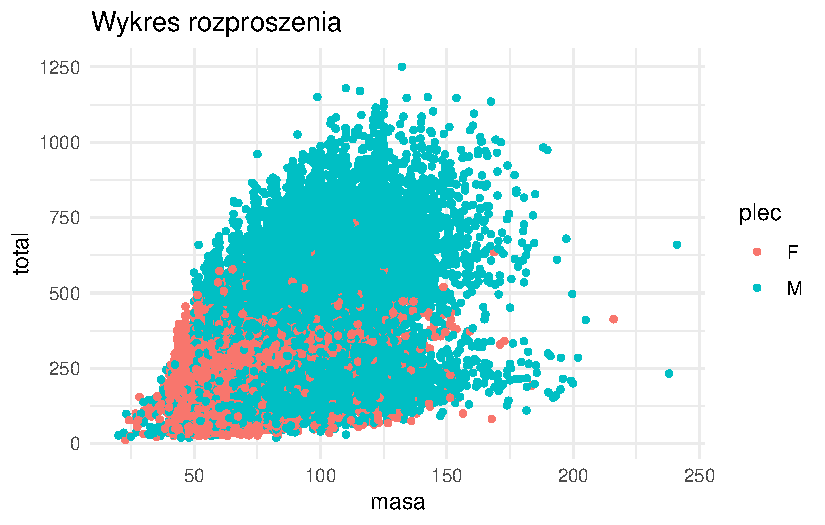
\includegraphics{raport_files/figure-pdf/unnamed-chunk-20-1.pdf}

}

\caption{Wykres rozproszenia wyniku total względem masy}

\end{figure}

Celem lepszej analizy zależności dokonamy teraz uśrednienia zmiennej
\textbf{Total} po zawodnikach tej samej płci o tej samej masie.

\begin{Shaded}
\begin{Highlighting}[]
\NormalTok{probka\_mean }\OtherTok{\textless{}{-}}\NormalTok{ probka }\SpecialCharTok{\%\textgreater{}\%}
  \FunctionTok{group\_by}\NormalTok{(masa, plec) }\SpecialCharTok{\%\textgreater{}\%}
  \FunctionTok{mutate}\NormalTok{(}\AttributeTok{mean\_total =} \FunctionTok{mean}\NormalTok{(total))}

\CommentTok{\# Keep only unique values of "masa"}
\NormalTok{probka\_mean\_unique }\OtherTok{\textless{}{-}}\NormalTok{ probka\_mean }\SpecialCharTok{\%\textgreater{}\%}
  \FunctionTok{distinct}\NormalTok{(masa, }\AttributeTok{.keep\_all =} \ConstantTok{TRUE}\NormalTok{)}

\CommentTok{\# Scatter plot with color by "plec" and mean points}
\FunctionTok{ggplot}\NormalTok{(probka\_mean\_unique, }\FunctionTok{aes}\NormalTok{(}\AttributeTok{x =}\NormalTok{ masa, }\AttributeTok{y =}\NormalTok{ mean\_total, }\AttributeTok{color =}\NormalTok{ plec)) }\SpecialCharTok{+}
  \FunctionTok{geom\_point}\NormalTok{(}\AttributeTok{size =} \DecValTok{3}\NormalTok{) }\SpecialCharTok{+}
  \FunctionTok{labs}\NormalTok{(}\AttributeTok{title =} \StringTok{"Scatter Plot of masa vs mean\_total"}\NormalTok{,}
       \AttributeTok{x =} \StringTok{"masa"}\NormalTok{, }\AttributeTok{y =} \StringTok{"mean\_total"}\NormalTok{, }\AttributeTok{color =} \StringTok{"Gender"}\NormalTok{) }\SpecialCharTok{+}
  \FunctionTok{theme\_minimal}\NormalTok{()}
\end{Highlighting}
\end{Shaded}

\begin{figure}[H]

{\centering 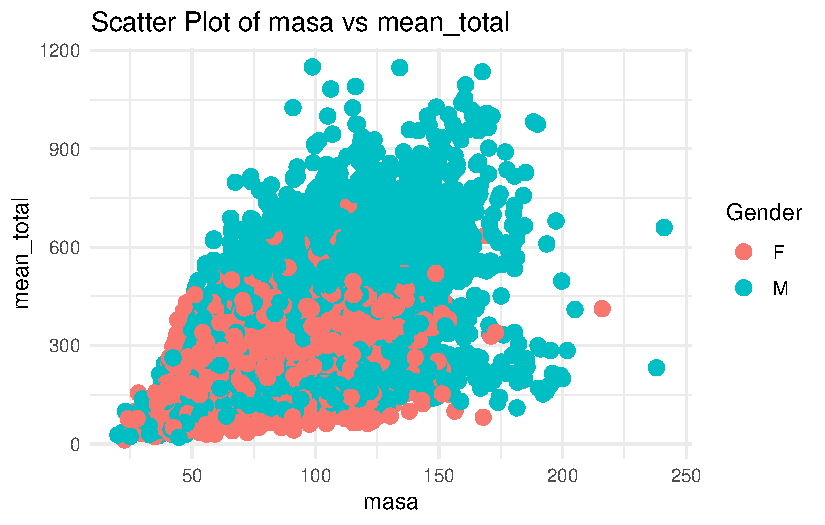
\includegraphics{raport_files/figure-pdf/unnamed-chunk-21-1.pdf}

}

\caption{Wykres rozproszenia po uśrednieniu po masie}

\end{figure}

Współczynniki korelacji pearsona dla całej populacji oraz dla każdej
płci z osobna prezentują się następująco.

\begin{Shaded}
\begin{Highlighting}[]
\NormalTok{cor\_by\_plec }\OtherTok{\textless{}{-}}\NormalTok{ probka\_mean\_unique }\SpecialCharTok{\%\textgreater{}\%}
  \FunctionTok{group\_by}\NormalTok{(plec) }\SpecialCharTok{\%\textgreater{}\%}
  \FunctionTok{summarize}\NormalTok{(}\AttributeTok{correlation =} \FunctionTok{cor}\NormalTok{(masa, total, }\AttributeTok{use =} \StringTok{"complete.obs"}\NormalTok{))}

\CommentTok{\# Calculate correlation for the entire data frame}
\NormalTok{cor\_total }\OtherTok{\textless{}{-}} \FunctionTok{cor}\NormalTok{(probka\_mean\_unique}\SpecialCharTok{$}\NormalTok{masa, probka\_mean\_unique}\SpecialCharTok{$}\NormalTok{total, }\AttributeTok{use =} \StringTok{"complete.obs"}\NormalTok{)}

\CommentTok{\# Print the results}
\FunctionTok{cat}\NormalTok{(}\StringTok{"Korelacja pomiędzy masą a wynikiem dla każdej z płci:}\SpecialCharTok{\textbackslash{}n}\StringTok{"}\NormalTok{)}
\end{Highlighting}
\end{Shaded}

\begin{verbatim}
Korelacja pomiędzy masą a wynikiem dla każdej z płci:
\end{verbatim}

\begin{Shaded}
\begin{Highlighting}[]
\FunctionTok{print}\NormalTok{(cor\_by\_plec)}
\end{Highlighting}
\end{Shaded}

\begin{verbatim}
# A tibble: 2 x 2
  plec  correlation
  <fct>       <dbl>
1 F           0.350
2 M           0.378
\end{verbatim}

\begin{Shaded}
\begin{Highlighting}[]
\FunctionTok{cat}\NormalTok{(}\StringTok{"Korelacja pomiędzy masą a wynikiem dla całej próbki:}\SpecialCharTok{\textbackslash{}n}\StringTok{"}\NormalTok{)}
\end{Highlighting}
\end{Shaded}

\begin{verbatim}
Korelacja pomiędzy masą a wynikiem dla całej próbki:
\end{verbatim}

\begin{Shaded}
\begin{Highlighting}[]
\FunctionTok{print}\NormalTok{(cor\_total)}
\end{Highlighting}
\end{Shaded}

\begin{verbatim}
[1] 0.4444799
\end{verbatim}

Na podstawie powyższych wartości można stwierdzić, że istnieją
przesłanki ku stwierdzeniu dodatniej korelacji pomiędzy masą ciała
zawodnika a jego wynikami siłowymi niezależnie od płci.

\hypertarget{podsumowanie}{%
\section{6. Podsumowanie}\label{podsumowanie}}

W wyniku powyższej analizy doszliśmy do następujących wniosków

\begin{itemize}
\item
  Rozkłady wyników siłowych dla poszczególnych płci cechują się
  \textbf{bimodalnością.} Nie byliśmy w stanie stwierdzić z czego ona
  wynika lecz przypuszczamy, że może mieć związek z grupą zawodników,
  którym nie udało się uzyskać poprawnego podejścia do któregoś z bojów
  przez co uzyskali oni wynik znacznie niższy niż większość.
\item
  Rozkłady masy zawodnika w niskich klasach wiekowych cechują się
  \textbf{leptokurtycznością i prawoskośnością.} Obserwujemy wiele
  wartości skrajnych oraz prawy ogon jest o wiele dłuższy od lewego.
  Zawodnikom młodym o wiele łatwiej jest utrzymywać wysoką masę ciała
  jednocześnie uzyskując dobre wyniki siłowe. \textbf{Stanowi to
  przesłankę ku dodatniej korelacji wyników siłowych i masy ciała.}
\item
  Rozkłady warunkowe wyników total cechują się \textbf{skośnością
  prawostronną,} która zwiększa się wraz z wiekiem. Również od pewnego
  momentu (\textbf{20-23)} wraz z wiekiem \textbf{maleje mediana.} Można
  więc pokusić się o stwierdzenie, że wtedy największa ilość zawodników
  przeżywa swój szczyt możliwości.
\item
  Masa zawodnika i jego osiągi siłowe są \textbf{dodatnio skorelowane.}
  Zgadza się to z naszą intuicją jak i poprzednimi obserwacjami.
  Uzasadnia to również dzielenie zawodników na kategorie wagowe jak ma
  to miejsce w przypadku większości zawodów.
\end{itemize}



\end{document}
